\documentclass[1p]{elsarticle_modified}
%\bibliographystyle{elsarticle-num}

%\usepackage[colorlinks]{hyperref}
%\usepackage{abbrmath_seonhwa} %\Abb, \Ascr, \Acal ,\Abf, \Afrak
\usepackage{amsfonts}
\usepackage{amssymb}
\usepackage{amsmath}
\usepackage{amsthm}
\usepackage{scalefnt}
\usepackage{amsbsy}
\usepackage{kotex}
\usepackage{caption}
\usepackage{subfig}
\usepackage{color}
\usepackage{graphicx}
\usepackage{xcolor} %% white, black, red, green, blue, cyan, magenta, yellow
\usepackage{float}
\usepackage{setspace}
\usepackage{hyperref}

\usepackage{tikz}
\usetikzlibrary{arrows}

\usepackage{multirow}
\usepackage{array} % fixed length table
\usepackage{hhline}

%%%%%%%%%%%%%%%%%%%%%
\makeatletter
\renewcommand*\env@matrix[1][\arraystretch]{%
	\edef\arraystretch{#1}%
	\hskip -\arraycolsep
	\let\@ifnextchar\new@ifnextchar
	\array{*\c@MaxMatrixCols c}}
\makeatother %https://tex.stackexchange.com/questions/14071/how-can-i-increase-the-line-spacing-in-a-matrix
%%%%%%%%%%%%%%%

\usepackage[normalem]{ulem}

\newcommand{\msout}[1]{\ifmmode\text{\sout{\ensuremath{#1}}}\else\sout{#1}\fi}
%SOURCE: \msout is \stkout macro in https://tex.stackexchange.com/questions/20609/strikeout-in-math-mode

\newcommand{\cancel}[1]{
	\ifmmode
	{\color{red}\msout{#1}}
	\else
	{\color{red}\sout{#1}}
	\fi
}

\newcommand{\add}[1]{
	{\color{blue}\uwave{#1}}
}

\newcommand{\replace}[2]{
	\ifmmode
	{\color{red}\msout{#1}}{\color{blue}\uwave{#2}}
	\else
	{\color{red}\sout{#1}}{\color{blue}\uwave{#2}}
	\fi
}

\newcommand{\Sol}{\mathcal{S}} %segment
\newcommand{\D}{D} %diagram
\newcommand{\A}{\mathcal{A}} %arc


%%%%%%%%%%%%%%%%%%%%%%%%%%%%%5 test

\def\sl{\operatorname{\textup{SL}}(2,\Cbb)}
\def\psl{\operatorname{\textup{PSL}}(2,\Cbb)}
\def\quan{\mkern 1mu \triangleright \mkern 1mu}

\theoremstyle{definition}
\newtheorem{thm}{Theorem}[section]
\newtheorem{prop}[thm]{Proposition}
\newtheorem{lem}[thm]{Lemma}
\newtheorem{ques}[thm]{Question}
\newtheorem{cor}[thm]{Corollary}
\newtheorem{defn}[thm]{Definition}
\newtheorem{exam}[thm]{Example}
\newtheorem{rmk}[thm]{Remark}
\newtheorem{alg}[thm]{Algorithm}

\newcommand{\I}{\sqrt{-1}}
\begin{document}

%\begin{frontmatter}
%
%\title{Boundary parabolic representations of knots up to 8 crossings}
%
%%% Group authors per affiliation:
%\author{Yunhi Cho} 
%\address{Department of Mathematics, University of Seoul, Seoul, Korea}
%\ead{yhcho@uos.ac.kr}
%
%
%\author{Seonhwa Kim} %\fnref{s_kim}}
%\address{Center for Geometry and Physics, Institute for Basic Science, Pohang, 37673, Korea}
%\ead{ryeona17@ibs.re.kr}
%
%\author{Hyuk Kim}
%\address{Department of Mathematical Sciences, Seoul National University, Seoul 08826, Korea}
%\ead{hyukkim@snu.ac.kr}
%
%\author{Seokbeom Yoon}
%\address{Department of Mathematical Sciences, Seoul National University, Seoul, 08826,  Korea}
%\ead{sbyoon15@snu.ac.kr}
%
%\begin{abstract}
%We find all boundary parabolic representation of knots up to 8 crossings.
%
%\end{abstract}
%\begin{keyword}
%    \MSC[2010] 57M25 
%\end{keyword}
%
%\end{frontmatter}

%\linenumbers
%\tableofcontents
%
\newcommand\colored[1]{\textcolor{white}{\rule[-0.35ex]{0.8em}{1.4ex}}\kern-0.8em\color{red} #1}%
%\newcommand\colored[1]{\textcolor{white}{ #1}\kern-2.17ex	\textcolor{white}{ #1}\kern-1.81ex	\textcolor{white}{ #1}\kern-2.15ex\color{red}#1	}

{\Large $\underline{12a_{0550}~(K12a_{0550})}$}

\setlength{\tabcolsep}{10pt}
\renewcommand{\arraystretch}{1.6}
\vspace{1cm}\begin{tabular}{m{100pt}>{\centering\arraybackslash}m{274pt}}
\multirow{5}{120pt}{
	\centering
	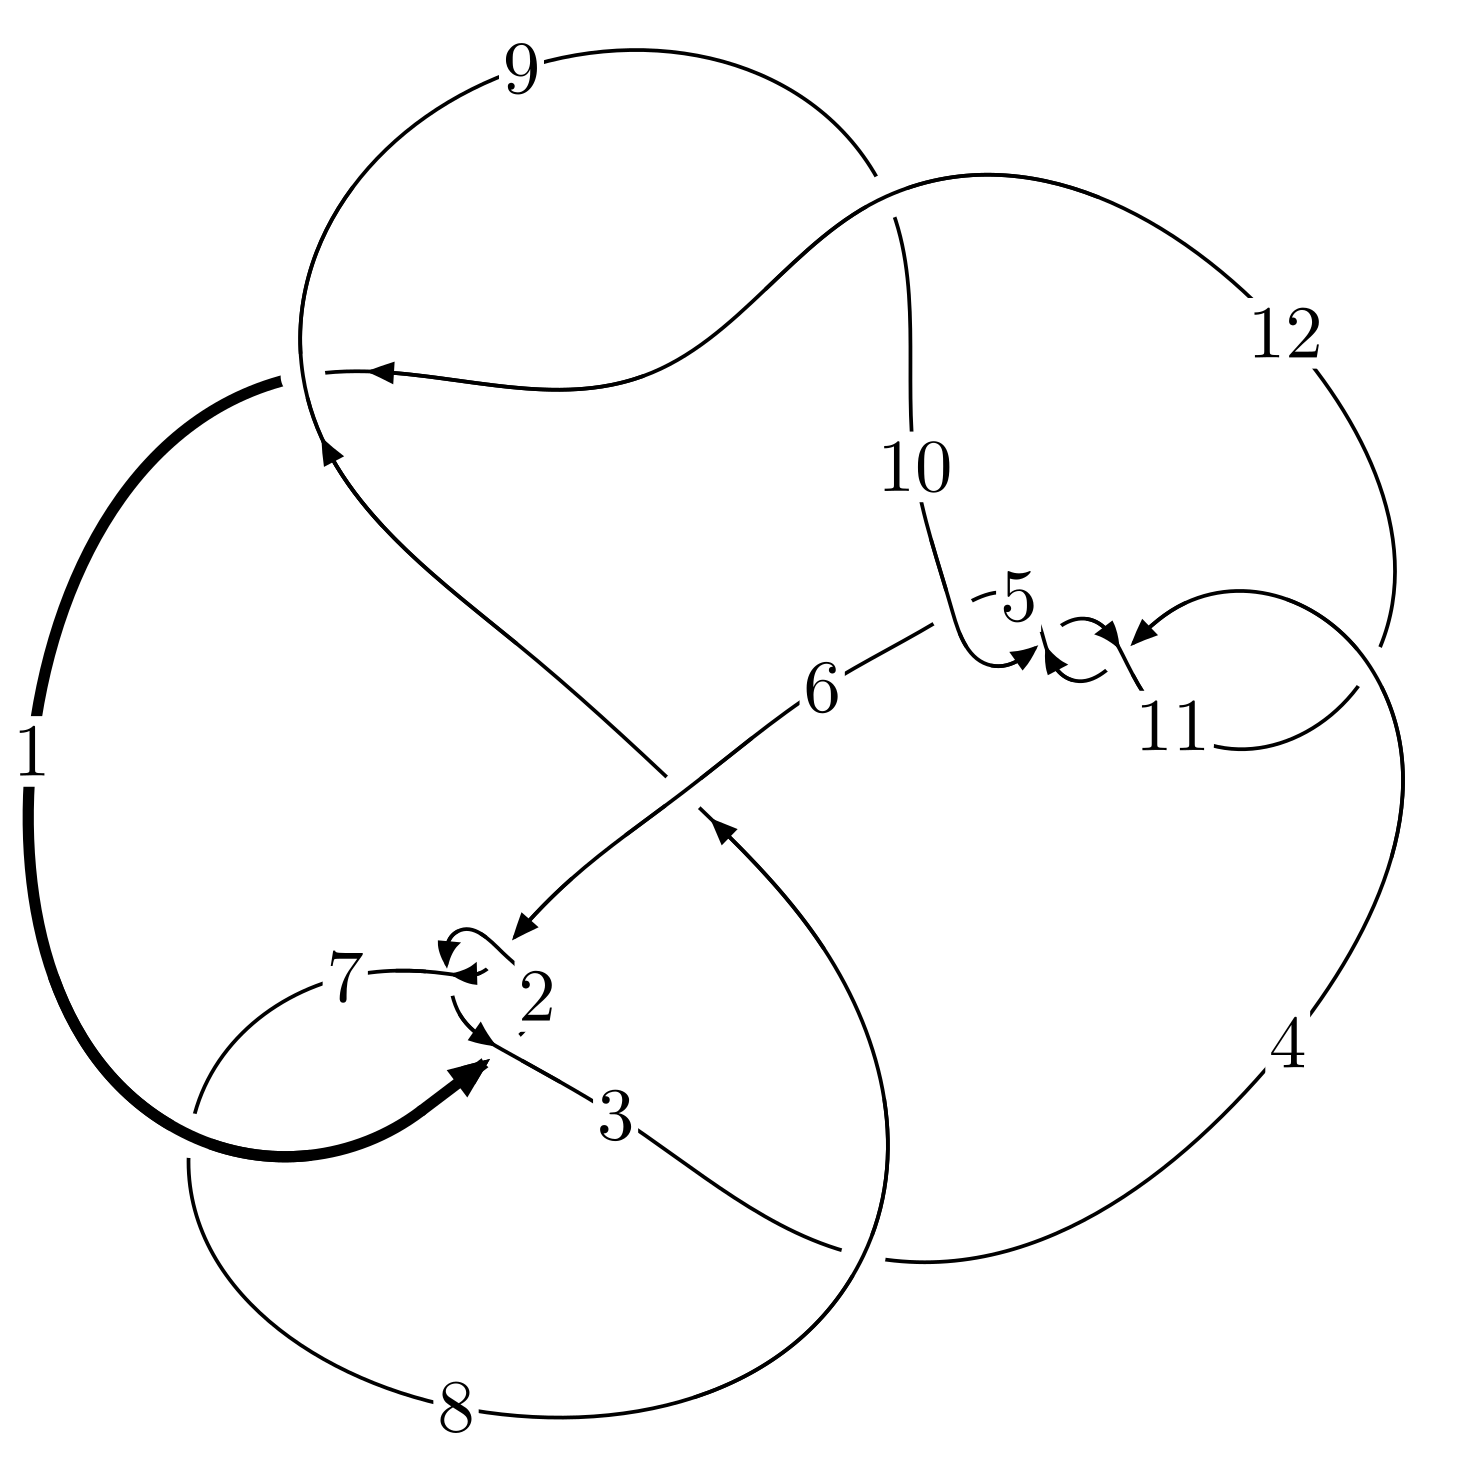
\includegraphics[width=112pt]{../../../GIT/diagram.site/Diagrams/png/1351_12a_0550.png}\\
\ \ \ A knot diagram\footnotemark}&
\allowdisplaybreaks
\textbf{Linearized knot diagam} \\
\cline{2-2}
 &
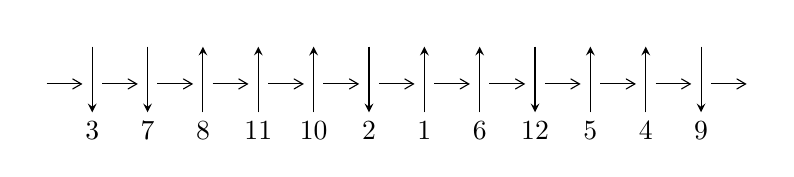
\begin{tikzpicture}[x=20pt, y=17pt]
	% nodes
	\node (C0) at (0, 0) {};
	\node (C1) at (1, 0) {};
	\node (C1U) at (1, +1) {};
	\node (C1D) at (1, -1) {3};

	\node (C2) at (2, 0) {};
	\node (C2U) at (2, +1) {};
	\node (C2D) at (2, -1) {7};

	\node (C3) at (3, 0) {};
	\node (C3U) at (3, +1) {};
	\node (C3D) at (3, -1) {8};

	\node (C4) at (4, 0) {};
	\node (C4U) at (4, +1) {};
	\node (C4D) at (4, -1) {11};

	\node (C5) at (5, 0) {};
	\node (C5U) at (5, +1) {};
	\node (C5D) at (5, -1) {10};

	\node (C6) at (6, 0) {};
	\node (C6U) at (6, +1) {};
	\node (C6D) at (6, -1) {2};

	\node (C7) at (7, 0) {};
	\node (C7U) at (7, +1) {};
	\node (C7D) at (7, -1) {1};

	\node (C8) at (8, 0) {};
	\node (C8U) at (8, +1) {};
	\node (C8D) at (8, -1) {6};

	\node (C9) at (9, 0) {};
	\node (C9U) at (9, +1) {};
	\node (C9D) at (9, -1) {12};

	\node (C10) at (10, 0) {};
	\node (C10U) at (10, +1) {};
	\node (C10D) at (10, -1) {5};

	\node (C11) at (11, 0) {};
	\node (C11U) at (11, +1) {};
	\node (C11D) at (11, -1) {4};

	\node (C12) at (12, 0) {};
	\node (C12U) at (12, +1) {};
	\node (C12D) at (12, -1) {9};
	\node (C13) at (13, 0) {};

	% arrows
	\draw[->,>={angle 60}]
	(C0) edge (C1) (C1) edge (C2) (C2) edge (C3) (C3) edge (C4) (C4) edge (C5) (C5) edge (C6) (C6) edge (C7) (C7) edge (C8) (C8) edge (C9) (C9) edge (C10) (C10) edge (C11) (C11) edge (C12) (C12) edge (C13) ;	\draw[->,>=stealth]
	(C1U) edge (C1D) (C2U) edge (C2D) (C3D) edge (C3U) (C4D) edge (C4U) (C5D) edge (C5U) (C6U) edge (C6D) (C7D) edge (C7U) (C8D) edge (C8U) (C9U) edge (C9D) (C10D) edge (C10U) (C11D) edge (C11U) (C12U) edge (C12D) ;
	\end{tikzpicture} \\
\hhline{~~} \\& 
\textbf{Solving Sequence} \\ \cline{2-2} 
 &
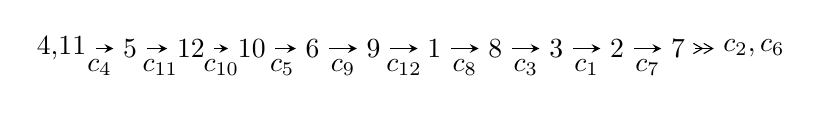
\begin{tikzpicture}[x=22pt, y=7pt]
	% node
	\node (A0) at (-1/8, 0) {4,11};
	\node (A1) at (1, 0) {5};
	\node (A2) at (2, 0) {12};
	\node (A3) at (3, 0) {10};
	\node (A4) at (4, 0) {6};
	\node (A5) at (5, 0) {9};
	\node (A6) at (6, 0) {1};
	\node (A7) at (7, 0) {8};
	\node (A8) at (8, 0) {3};
	\node (A9) at (9, 0) {2};
	\node (A10) at (10, 0) {7};
	\node (C1) at (1/2, -1) {$c_{4}$};
	\node (C2) at (3/2, -1) {$c_{11}$};
	\node (C3) at (5/2, -1) {$c_{10}$};
	\node (C4) at (7/2, -1) {$c_{5}$};
	\node (C5) at (9/2, -1) {$c_{9}$};
	\node (C6) at (11/2, -1) {$c_{12}$};
	\node (C7) at (13/2, -1) {$c_{8}$};
	\node (C8) at (15/2, -1) {$c_{3}$};
	\node (C9) at (17/2, -1) {$c_{1}$};
	\node (C10) at (19/2, -1) {$c_{7}$};
	\node (A11) at (45/4, 0) {$c_{2},c_{6}$};

	% edge
	\draw[->,>=stealth]	
	(A0) edge (A1) (A1) edge (A2) (A2) edge (A3) (A3) edge (A4) (A4) edge (A5) (A5) edge (A6) (A6) edge (A7) (A7) edge (A8) (A8) edge (A9) (A9) edge (A10) ;
	\draw[->>,>={angle 60}]	
	(A10) edge (A11);
\end{tikzpicture} \\ 

\end{tabular} \\

\footnotetext{
The image of knot diagram is generated by the software ``\textbf{Draw programme}" developed by Andrew Bartholomew(\url{http://www.layer8.co.uk/maths/draw/index.htm\#Running-draw}), where we modified some parts for our purpose(\url{https://github.com/CATsTAILs/LinksPainter}).
}\phantom \\ \newline 
\centering \textbf{Ideals for irreducible components\footnotemark of $X_{\text{par}}$} 
 
\begin{align*}
I^u_{1}&=\langle 
u^{74}+u^{73}+\cdots+u+1\rangle \\
\\
\end{align*}
\raggedright * 1 irreducible components of $\dim_{\mathbb{C}}=0$, with total 74 representations.\\
\footnotetext{All coefficients of polynomials are rational numbers. But the coefficients are sometimes approximated in decimal forms when there is not enough margin.}
\newpage
\renewcommand{\arraystretch}{1}
\centering \section*{I. $I^u_{1}= \langle u^{74}+u^{73}+\cdots+u+1 \rangle$}
\flushleft \textbf{(i) Arc colorings}\\
\begin{tabular}{m{7pt} m{180pt} m{7pt} m{180pt} }
\flushright $a_{4}=$&$\begin{pmatrix}1\\0\end{pmatrix}$ \\
\flushright $a_{11}=$&$\begin{pmatrix}0\\u\end{pmatrix}$ \\
\flushright $a_{5}=$&$\begin{pmatrix}1\\- u^2\end{pmatrix}$ \\
\flushright $a_{12}=$&$\begin{pmatrix}u\\u\end{pmatrix}$ \\
\flushright $a_{10}=$&$\begin{pmatrix}- u\\u^3+u\end{pmatrix}$ \\
\flushright $a_{6}=$&$\begin{pmatrix}u^2+1\\- u^4-2 u^2\end{pmatrix}$ \\
\flushright $a_{9}=$&$\begin{pmatrix}u^5+2 u^3- u\\u^5+3 u^3+u\end{pmatrix}$ \\
\flushright $a_{1}=$&$\begin{pmatrix}u^9+4 u^7+3 u^5-2 u^3+u\\u^9+5 u^7+7 u^5+2 u^3+u\end{pmatrix}$ \\
\flushright $a_{8}=$&$\begin{pmatrix}- u^{11}-6 u^9-12 u^7-8 u^5- u^3-2 u\\u^{13}+7 u^{11}+17 u^9+16 u^7+6 u^5+5 u^3+u\end{pmatrix}$ \\
\flushright $a_{3}=$&$\begin{pmatrix}- u^{24}-13 u^{22}+\cdots-2 u^2+1\\u^{26}+14 u^{24}+\cdots+10 u^4+u^2\end{pmatrix}$ \\
\flushright $a_{2}=$&$\begin{pmatrix}- u^{59}-32 u^{57}+\cdots+28 u^5+u^3\\u^{61}+33 u^{59}+\cdots+u^3+u\end{pmatrix}$ \\
\flushright $a_{7}=$&$\begin{pmatrix}- u^{31}-16 u^{29}+\cdots-4 u^3-2 u\\- u^{31}-17 u^{29}+\cdots+2 u^3+u\end{pmatrix}$\\&\end{tabular}
\flushleft \textbf{(ii) Obstruction class $= -1$}\\~\\
\flushleft \textbf{(iii) Cusp Shapes $= 4 u^{73}+4 u^{72}+\cdots+4 u+2$}\\~\\
\newpage\renewcommand{\arraystretch}{1}
\flushleft \textbf{(iv) u-Polynomials at the component}\newline \\
\begin{tabular}{m{50pt}|m{274pt}}
Crossings & \hspace{64pt}u-Polynomials at each crossing \\
\hline $$\begin{aligned}c_{1}\end{aligned}$$&$\begin{aligned}
&u^{74}+35 u^{73}+\cdots- u+1
\end{aligned}$\\
\hline $$\begin{aligned}c_{2},c_{6}\end{aligned}$$&$\begin{aligned}
&u^{74}- u^{73}+\cdots- u+1
\end{aligned}$\\
\hline $$\begin{aligned}c_{3}\end{aligned}$$&$\begin{aligned}
&u^{74}+u^{73}+\cdots-879 u+481
\end{aligned}$\\
\hline $$\begin{aligned}c_{4},c_{5},c_{10}\\c_{11}\end{aligned}$$&$\begin{aligned}
&u^{74}- u^{73}+\cdots- u+1
\end{aligned}$\\
\hline $$\begin{aligned}c_{7}\end{aligned}$$&$\begin{aligned}
&u^{74}-3 u^{73}+\cdots-325 u+175
\end{aligned}$\\
\hline $$\begin{aligned}c_{8}\end{aligned}$$&$\begin{aligned}
&u^{74}+9 u^{73}+\cdots+169 u+13
\end{aligned}$\\
\hline $$\begin{aligned}c_{9},c_{12}\end{aligned}$$&$\begin{aligned}
&u^{74}-13 u^{73}+\cdots-2717 u+283
\end{aligned}$\\
\hline
\end{tabular}\\~\\
\newpage\renewcommand{\arraystretch}{1}
\flushleft \textbf{(v) Riley Polynomials at the component}\newline \\
\begin{tabular}{m{50pt}|m{274pt}}
Crossings & \hspace{64pt}Riley Polynomials at each crossing \\
\hline $$\begin{aligned}c_{1}\end{aligned}$$&$\begin{aligned}
&y^{74}+9 y^{73}+\cdots+5 y+1
\end{aligned}$\\
\hline $$\begin{aligned}c_{2},c_{6}\end{aligned}$$&$\begin{aligned}
&y^{74}-35 y^{73}+\cdots+y+1
\end{aligned}$\\
\hline $$\begin{aligned}c_{3}\end{aligned}$$&$\begin{aligned}
&y^{74}-19 y^{73}+\cdots-9331555 y+231361
\end{aligned}$\\
\hline $$\begin{aligned}c_{4},c_{5},c_{10}\\c_{11}\end{aligned}$$&$\begin{aligned}
&y^{74}+81 y^{73}+\cdots+y+1
\end{aligned}$\\
\hline $$\begin{aligned}c_{7}\end{aligned}$$&$\begin{aligned}
&y^{74}+17 y^{73}+\cdots+1185525 y+30625
\end{aligned}$\\
\hline $$\begin{aligned}c_{8}\end{aligned}$$&$\begin{aligned}
&y^{74}+5 y^{73}+\cdots+4433 y+169
\end{aligned}$\\
\hline $$\begin{aligned}c_{9},c_{12}\end{aligned}$$&$\begin{aligned}
&y^{74}+45 y^{73}+\cdots+403241 y+80089
\end{aligned}$\\
\hline
\end{tabular}\\~\\
\newpage\flushleft \textbf{(vi) Complex Volumes and Cusp Shapes}
$$\begin{array}{c|c|c}  
\text{Solutions to }I^u_{1}& \I (\text{vol} + \sqrt{-1}CS) & \text{Cusp shape}\\
 \hline 
\begin{aligned}
u &= -0.581679 + 0.588687 I\end{aligned}
 & \phantom{-}1.14751 - 12.21490 I & \phantom{-}2.00000 + 10.62461 I \\ \hline\begin{aligned}
u &= -0.581679 - 0.588687 I\end{aligned}
 & \phantom{-}1.14751 + 12.21490 I & \phantom{-}2.00000 - 10.62461 I \\ \hline\begin{aligned}
u &= \phantom{-}0.579078 + 0.579968 I\end{aligned}
 & \phantom{-}3.39034 + 7.17138 I & \phantom{-}4.72098 - 6.80374 I \\ \hline\begin{aligned}
u &= \phantom{-}0.579078 - 0.579968 I\end{aligned}
 & \phantom{-}3.39034 - 7.17138 I & \phantom{-}4.72098 + 6.80374 I \\ \hline\begin{aligned}
u &= -0.558960 + 0.584212 I\end{aligned}
 & -1.22103 - 4.59999 I & -1.85198 + 5.42057 I \\ \hline\begin{aligned}
u &= -0.558960 - 0.584212 I\end{aligned}
 & -1.22103 + 4.59999 I & -1.85198 - 5.42057 I \\ \hline\begin{aligned}
u &= \phantom{-}0.580042 + 0.552186 I\end{aligned}
 & \phantom{-}4.60737 + 4.92092 I & \phantom{-}6.44482 - 6.98206 I \\ \hline\begin{aligned}
u &= \phantom{-}0.580042 - 0.552186 I\end{aligned}
 & \phantom{-}4.60737 - 4.92092 I & \phantom{-}6.44482 + 6.98206 I \\ \hline\begin{aligned}
u &= -0.581910 + 0.533281 I\end{aligned}
 & \phantom{-}3.51551 - 0.09713 I & \phantom{-}4.79421 + 0.95551 I \\ \hline\begin{aligned}
u &= -0.581910 - 0.533281 I\end{aligned}
 & \phantom{-}3.51551 + 0.09713 I & \phantom{-}4.79421 - 0.95551 I \\ \hline\begin{aligned}
u &= \phantom{-}0.160664 + 0.764547 I\end{aligned}
 & -3.59023 + 7.24183 I & -4.81965 - 8.01497 I \\ \hline\begin{aligned}
u &= \phantom{-}0.160664 - 0.764547 I\end{aligned}
 & -3.59023 - 7.24183 I & -4.81965 + 8.01497 I \\ \hline\begin{aligned}
u &= \phantom{-}0.081400 + 0.760927 I\end{aligned}
 & -5.25802 - 0.19086 I & -8.37896 - 0.60569 I \\ \hline\begin{aligned}
u &= \phantom{-}0.081400 - 0.760927 I\end{aligned}
 & -5.25802 + 0.19086 I & -8.37896 + 0.60569 I \\ \hline\begin{aligned}
u &= \phantom{-}0.475714 + 0.583485 I\end{aligned}
 & -2.85675 + 4.95140 I & -3.45849 - 7.85168 I \\ \hline\begin{aligned}
u &= \phantom{-}0.475714 - 0.583485 I\end{aligned}
 & -2.85675 - 4.95140 I & -3.45849 + 7.85168 I \\ \hline\begin{aligned}
u &= -0.594230 + 0.443922 I\end{aligned}
 & \phantom{-}3.77889 - 3.92096 I & \phantom{-}5.61393 + 5.93891 I \\ \hline\begin{aligned}
u &= -0.594230 - 0.443922 I\end{aligned}
 & \phantom{-}3.77889 + 3.92096 I & \phantom{-}5.61393 - 5.93891 I \\ \hline\begin{aligned}
u &= -0.149812 + 0.724787 I\end{aligned}
 & -1.30291 - 2.53624 I & -1.75249 + 4.49036 I \\ \hline\begin{aligned}
u &= -0.149812 - 0.724787 I\end{aligned}
 & -1.30291 + 2.53624 I & -1.75249 - 4.49036 I \\ \hline\begin{aligned}
u &= \phantom{-}0.595573 + 0.422112 I\end{aligned}
 & \phantom{-}4.98992 - 0.90435 I & \phantom{-}7.85161 + 0.13371 I \\ \hline\begin{aligned}
u &= \phantom{-}0.595573 - 0.422112 I\end{aligned}
 & \phantom{-}4.98992 + 0.90435 I & \phantom{-}7.85161 - 0.13371 I \\ \hline\begin{aligned}
u &= -0.611496 + 0.376425 I\end{aligned}
 & \phantom{-}1.77025 + 8.14990 I & \phantom{-}3.28357 - 4.51693 I \\ \hline\begin{aligned}
u &= -0.611496 - 0.376425 I\end{aligned}
 & \phantom{-}1.77025 - 8.14990 I & \phantom{-}3.28357 + 4.51693 I \\ \hline\begin{aligned}
u &= \phantom{-}0.603907 + 0.386844 I\end{aligned}
 & \phantom{-}3.95690 - 3.13486 I & \phantom{-}6.57615 + 0.47238 I \\ \hline\begin{aligned}
u &= \phantom{-}0.603907 - 0.386844 I\end{aligned}
 & \phantom{-}3.95690 + 3.13486 I & \phantom{-}6.57615 - 0.47238 I \\ \hline\begin{aligned}
u &= \phantom{-}0.384733 + 0.589181 I\end{aligned}
 & -2.15217 - 2.34776 I & -2.61549 - 0.50712 I \\ \hline\begin{aligned}
u &= \phantom{-}0.384733 - 0.589181 I\end{aligned}
 & -2.15217 + 2.34776 I & -2.61549 + 0.50712 I \\ \hline\begin{aligned}
u &= -0.457206 + 0.515716 I\end{aligned}
 & \phantom{-}0.32851 - 1.59321 I & \phantom{-}1.85928 + 4.31200 I \\ \hline\begin{aligned}
u &= -0.457206 - 0.515716 I\end{aligned}
 & \phantom{-}0.32851 + 1.59321 I & \phantom{-}1.85928 - 4.31200 I\\
 \hline 
 \end{array}$$\newpage$$\begin{array}{c|c|c}  
\text{Solutions to }I^u_{1}& \I (\text{vol} + \sqrt{-1}CS) & \text{Cusp shape}\\
 \hline 
\begin{aligned}
u &= -0.576050 + 0.370037 I\end{aligned}
 & -0.597920 + 0.702387 I & \phantom{-}0.117490 + 1.017971 I \\ \hline\begin{aligned}
u &= -0.576050 - 0.370037 I\end{aligned}
 & -0.597920 - 0.702387 I & \phantom{-}0.117490 - 1.017971 I \\ \hline\begin{aligned}
u &= -0.191536 + 0.572330 I\end{aligned}
 & -0.30101 - 1.44762 I & -0.21354 + 6.41359 I \\ \hline\begin{aligned}
u &= -0.191536 - 0.572330 I\end{aligned}
 & -0.30101 + 1.44762 I & -0.21354 - 6.41359 I \\ \hline\begin{aligned}
u &= -0.13095 + 1.44541 I\end{aligned}
 & -4.02653 + 5.58703 I & \phantom{-0.000000 } 0 \\ \hline\begin{aligned}
u &= -0.13095 - 1.44541 I\end{aligned}
 & -4.02653 - 5.58703 I & \phantom{-0.000000 } 0 \\ \hline\begin{aligned}
u &= \phantom{-}0.13429 + 1.45675 I\end{aligned}
 & -1.94463 - 0.59547 I & \phantom{-0.000000 } 0 \\ \hline\begin{aligned}
u &= \phantom{-}0.13429 - 1.45675 I\end{aligned}
 & -1.94463 + 0.59547 I & \phantom{-0.000000 } 0 \\ \hline\begin{aligned}
u &= -0.10830 + 1.47365 I\end{aligned}
 & -6.49129 - 1.54826 I & \phantom{-0.000000 } 0 \\ \hline\begin{aligned}
u &= -0.10830 - 1.47365 I\end{aligned}
 & -6.49129 + 1.54826 I & \phantom{-0.000000 } 0 \\ \hline\begin{aligned}
u &= \phantom{-}0.14890 + 1.47840 I\end{aligned}
 & -1.17433 + 1.68063 I & \phantom{-0.000000 } 0 \\ \hline\begin{aligned}
u &= \phantom{-}0.14890 - 1.47840 I\end{aligned}
 & -1.17433 - 1.68063 I & \phantom{-0.000000 } 0 \\ \hline\begin{aligned}
u &= \phantom{-}0.442216 + 0.250522 I\end{aligned}
 & -2.00759 - 1.71991 I & -0.002985 + 0.493302 I \\ \hline\begin{aligned}
u &= \phantom{-}0.442216 - 0.250522 I\end{aligned}
 & -2.00759 + 1.71991 I & -0.002985 - 0.493302 I \\ \hline\begin{aligned}
u &= -0.15679 + 1.48846 I\end{aligned}
 & -2.52069 - 6.55186 I & \phantom{-0.000000 } 0 \\ \hline\begin{aligned}
u &= -0.15679 - 1.48846 I\end{aligned}
 & -2.52069 + 6.55186 I & \phantom{-0.000000 } 0 \\ \hline\begin{aligned}
u &= \phantom{-}0.465321 + 0.114222 I\end{aligned}
 & -0.77170 + 5.14412 I & \phantom{-}3.35203 - 6.10091 I \\ \hline\begin{aligned}
u &= \phantom{-}0.465321 - 0.114222 I\end{aligned}
 & -0.77170 - 5.14412 I & \phantom{-}3.35203 + 6.10091 I \\ \hline\begin{aligned}
u &= -0.16980 + 1.53508 I\end{aligned}
 & -3.33883 - 2.79785 I & \phantom{-0.000000 } 0 \\ \hline\begin{aligned}
u &= -0.16980 - 1.53508 I\end{aligned}
 & -3.33883 + 2.79785 I & \phantom{-0.000000 } 0 \\ \hline\begin{aligned}
u &= -0.02101 + 1.54796 I\end{aligned}
 & -7.42999 - 2.03723 I & \phantom{-0.000000 } 0 \\ \hline\begin{aligned}
u &= -0.02101 - 1.54796 I\end{aligned}
 & -7.42999 + 2.03723 I & \phantom{-0.000000 } 0 \\ \hline\begin{aligned}
u &= -0.13143 + 1.54609 I\end{aligned}
 & -6.62453 - 3.70192 I & \phantom{-0.000000 } 0 \\ \hline\begin{aligned}
u &= -0.13143 - 1.54609 I\end{aligned}
 & -6.62453 + 3.70192 I & \phantom{-0.000000 } 0 \\ \hline\begin{aligned}
u &= \phantom{-}0.17209 + 1.54345 I\end{aligned}
 & -2.35401 + 7.64003 I & \phantom{-0.000000 } 0 \\ \hline\begin{aligned}
u &= \phantom{-}0.17209 - 1.54345 I\end{aligned}
 & -2.35401 - 7.64003 I & \phantom{-0.000000 } 0 \\ \hline\begin{aligned}
u &= \phantom{-}0.11928 + 1.55708 I\end{aligned}
 & -9.35786 - 0.47227 I & \phantom{-0.000000 } 0 \\ \hline\begin{aligned}
u &= \phantom{-}0.11928 - 1.55708 I\end{aligned}
 & -9.35786 + 0.47227 I & \phantom{-0.000000 } 0 \\ \hline\begin{aligned}
u &= \phantom{-}0.17433 + 1.55520 I\end{aligned}
 & -3.72276 + 9.91652 I & \phantom{-0.000000 } 0 \\ \hline\begin{aligned}
u &= \phantom{-}0.17433 - 1.55520 I\end{aligned}
 & -3.72276 - 9.91652 I & \phantom{-0.000000 } 0\\
 \hline 
 \end{array}$$\newpage$$\begin{array}{c|c|c}  
\text{Solutions to }I^u_{1}& \I (\text{vol} + \sqrt{-1}CS) & \text{Cusp shape}\\
 \hline 
\begin{aligned}
u &= \phantom{-}0.13939 + 1.55951 I\end{aligned}
 & -10.05520 + 7.19221 I & \phantom{-0.000000 } 0 \\ \hline\begin{aligned}
u &= \phantom{-}0.13939 - 1.55951 I\end{aligned}
 & -10.05520 - 7.19221 I & \phantom{-0.000000 } 0 \\ \hline\begin{aligned}
u &= -0.16695 + 1.55795 I\end{aligned}
 & -8.37394 - 7.24510 I & \phantom{-0.000000 } 0 \\ \hline\begin{aligned}
u &= -0.16695 - 1.55795 I\end{aligned}
 & -8.37394 + 7.24510 I & \phantom{-0.000000 } 0 \\ \hline\begin{aligned}
u &= -0.17594 + 1.55858 I\end{aligned}
 & -6.0096 - 14.9821 I & \phantom{-0.000000 } 0 \\ \hline\begin{aligned}
u &= -0.17594 - 1.55858 I\end{aligned}
 & -6.0096 + 14.9821 I & \phantom{-0.000000 } 0 \\ \hline\begin{aligned}
u &= -0.412346 + 0.073322 I\end{aligned}
 & \phantom{-}1.227240 - 0.638691 I & \phantom{-}7.97254 + 1.54143 I \\ \hline\begin{aligned}
u &= -0.412346 - 0.073322 I\end{aligned}
 & \phantom{-}1.227240 + 0.638691 I & \phantom{-}7.97254 - 1.54143 I \\ \hline\begin{aligned}
u &= -0.02854 + 1.58475 I\end{aligned}
 & -9.12688 - 3.11271 I & \phantom{-0.000000 } 0 \\ \hline\begin{aligned}
u &= -0.02854 - 1.58475 I\end{aligned}
 & -9.12688 + 3.11271 I & \phantom{-0.000000 } 0 \\ \hline\begin{aligned}
u &= \phantom{-}0.01619 + 1.59177 I\end{aligned}
 & -13.22470 + 0.12897 I & \phantom{-0.000000 } 0 \\ \hline\begin{aligned}
u &= \phantom{-}0.01619 - 1.59177 I\end{aligned}
 & -13.22470 - 0.12897 I & \phantom{-0.000000 } 0 \\ \hline\begin{aligned}
u &= \phantom{-}0.03179 + 1.59277 I\end{aligned}
 & -11.57340 + 7.87379 I & \phantom{-0.000000 } 0 \\ \hline\begin{aligned}
u &= \phantom{-}0.03179 - 1.59277 I\end{aligned}
 & -11.57340 - 7.87379 I & \phantom{-0.000000 } 0\\
 \hline 
 \end{array}$$\newpage
\newpage\renewcommand{\arraystretch}{1}
\centering \section*{ II. u-Polynomials}
\begin{tabular}{m{50pt}|m{274pt}}
Crossings & \hspace{64pt}u-Polynomials at each crossing \\
\hline $$\begin{aligned}c_{1}\end{aligned}$$&$\begin{aligned}
&u^{74}+35 u^{73}+\cdots- u+1
\end{aligned}$\\
\hline $$\begin{aligned}c_{2},c_{6}\end{aligned}$$&$\begin{aligned}
&u^{74}- u^{73}+\cdots- u+1
\end{aligned}$\\
\hline $$\begin{aligned}c_{3}\end{aligned}$$&$\begin{aligned}
&u^{74}+u^{73}+\cdots-879 u+481
\end{aligned}$\\
\hline $$\begin{aligned}c_{4},c_{5},c_{10}\\c_{11}\end{aligned}$$&$\begin{aligned}
&u^{74}- u^{73}+\cdots- u+1
\end{aligned}$\\
\hline $$\begin{aligned}c_{7}\end{aligned}$$&$\begin{aligned}
&u^{74}-3 u^{73}+\cdots-325 u+175
\end{aligned}$\\
\hline $$\begin{aligned}c_{8}\end{aligned}$$&$\begin{aligned}
&u^{74}+9 u^{73}+\cdots+169 u+13
\end{aligned}$\\
\hline $$\begin{aligned}c_{9},c_{12}\end{aligned}$$&$\begin{aligned}
&u^{74}-13 u^{73}+\cdots-2717 u+283
\end{aligned}$\\
\hline
\end{tabular}\newpage\renewcommand{\arraystretch}{1}
\centering \section*{ III. Riley Polynomials}
\begin{tabular}{m{50pt}|m{274pt}}
Crossings & \hspace{64pt}Riley Polynomials at each crossing \\
\hline $$\begin{aligned}c_{1}\end{aligned}$$&$\begin{aligned}
&y^{74}+9 y^{73}+\cdots+5 y+1
\end{aligned}$\\
\hline $$\begin{aligned}c_{2},c_{6}\end{aligned}$$&$\begin{aligned}
&y^{74}-35 y^{73}+\cdots+y+1
\end{aligned}$\\
\hline $$\begin{aligned}c_{3}\end{aligned}$$&$\begin{aligned}
&y^{74}-19 y^{73}+\cdots-9331555 y+231361
\end{aligned}$\\
\hline $$\begin{aligned}c_{4},c_{5},c_{10}\\c_{11}\end{aligned}$$&$\begin{aligned}
&y^{74}+81 y^{73}+\cdots+y+1
\end{aligned}$\\
\hline $$\begin{aligned}c_{7}\end{aligned}$$&$\begin{aligned}
&y^{74}+17 y^{73}+\cdots+1185525 y+30625
\end{aligned}$\\
\hline $$\begin{aligned}c_{8}\end{aligned}$$&$\begin{aligned}
&y^{74}+5 y^{73}+\cdots+4433 y+169
\end{aligned}$\\
\hline $$\begin{aligned}c_{9},c_{12}\end{aligned}$$&$\begin{aligned}
&y^{74}+45 y^{73}+\cdots+403241 y+80089
\end{aligned}$\\
\hline
\end{tabular}
\vskip 2pc
\end{document}